\documentclass{beamer}

\usepackage{amsfonts,amsmath,comment,graphicx,listings}

\title{Spectral Rigid Body Dynamics}
\author{Mikola Lysenko}

\begin{document}

\lstset{ %
language=Python,                % choose the language of the code
basicstyle=\footnotesize,       % the size of the fonts that are used for the code
showspaces=false,               % show spaces adding particular underscores
showstringspaces=false,         % underline spaces within strings
showtabs=false,                 % show tabs within strings adding particular underscores
frame=single,	                % adds a frame around the code
tabsize=4,	                % sets default tabsize to 2 spaces
captionpos=b,                   % sets the caption-position to bottom
breaklines=true,                % sets automatic line breaking
breakatwhitespace=false}

\newcommand{\R}{\mathbb{R}}
\newcommand{\ind}[1]{{\bf 1}_{#1}}
\newcommand{\inner}[2]{\left \langle #1 , #2 \right \rangle}
%\newcommand{\exp}{\mathop{\text{exp}}}

\maketitle

\begin{frame}
	\frametitle{Overview}
		\tableofcontents
\end{frame}

\section{Rigid Body Dynamics}
\begin{frame}
\frametitle{Rigid Body Dynamics}
An approximate model of low energy physics for stiff objects

\pause
\vskip15pt
Pros:
\begin{itemize}
	\item{+} Pretty accurate at human energy scales
	\item{+} Good for stiff materials (ie metals, plastics etc.)
	\item{+} Easy kinematic constraints (useful for mechanisms)
	\item{+} Standard animation tool (videogames!)
\end{itemize}

\pause
\vskip15pt
Cons:
\begin{itemize}
	\item{-} Inaccurate at extremely large energies
	\item{-} Bad for materials with low elastic modulus
	\item{-} Not always solvable! (See: Painleve's paradox)
\end{itemize}
\end{frame}

\begin{frame}
\frametitle{What is a Rigid Body?}
An idealized solid object with elastic modulus $= \infty$
\pause
\vskip5pt
We identify a body $B$ with a scalar field, $\varphi : \R^d \to \R^+$
\vskip5pt
\begin{center}
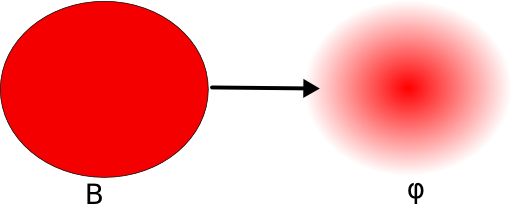
\includegraphics[height=1.1in]{figures/massfield.png}
\end{center}
\pause
\vskip5pt
$\varphi$ represents the mass distribution of $B$
\pause
\vskip5pt
$\varphi(x) = 0$ indicates $B$ does not occupy the space at $x$
\end{frame}

\begin{frame}
\frametitle{Configuration Space of a Rigid Body}
Transformations of rigid mass fields must preserve distance and handedness
\pause
\vskip5pt
In other words, must be a direct Euclidean isometry
\vskip5pt
Isomorphic to finite dimensional Lie group, $SE(d) \cong SO(d) \ltimes \R^d$
\vskip5pt
\pause
\begin{columns}
	\column{.5\textwidth}
		\begin{center}
		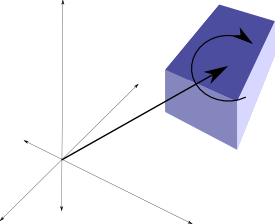
\includegraphics[height=1.4in]{figures/rigidbody.png}
		\end{center}
		
	\column{.5\textwidth}
		\begin{center}
		Can be parameterized by a translation $t$ and a rotation $R$
		
		\vskip15pt
		
		Matrix:
		$\left( \begin{array}{cc}
			R & t \\
			0 & 1 \\
		\end{array} \right)$
		
		\vskip15pt
		${d+1 \choose{2}}$ degrees of freedom
		
		\vskip15pt
		Tangent space: $\mathfrak{so}(d+1)$
		\end{center}
\end{columns}
\pause
\vskip10pt
\begin{center}
\bf{Motions of rigid objects $\cong$ curves $q(t) \subset SE(d)$}
\end{center}
\end{frame}


\section{Lagrangian Mechanics}
\begin{frame}
\frametitle{Lagrangian Mechanics}
Turns physics into an optimization problem.
\vskip5pt
\pause
Given a configuration curve $q$ at time $t$, define the \emph{Lagrangian}
\[ \mathcal{L}(q, \dot{q}, t) = T(\dot{q}) - U(q, t) \]
Where $T(\dot{q}) = \frac{1}{2} \dot{q}^T M \dot{q}$ is the kinetic energy and $U$ is a potential
\vskip15pt
\pause
{\bf Hamilton's Principle of Least Action}:
\begin{center}
	\emph{Physically plausible motions do minimal work}
\end{center}
\vskip10pt
\pause
In other words:
\[ \mathop{\text{argmin}}_{q : [t_0, t_1) \to SE(d)} \int \limits_{t_0}^{t_1} L(q, \dot{q}, t) dt \]
\end{frame}

\begin{frame}
\frametitle{Forward Kinematics}
Solve:
\[ \mathop{\text{argmin}}_{q : [t_0, t_1) \to SE(d)} \int \limits_{t_0}^{t_1} L(q, \dot{q}, t) dt \]
\pause
This is a 1st order variational problem, so use Euler-Lagrange:
\[ \frac{d}{dt} \left ( \frac{\partial L(q, \dot{q}, t)}{\partial \dot{q}} \right) = \frac{\partial L(q, \dot{q}, t)}{\partial q} \]
\pause
Unpack definitions and simplify:
\begin{eqnarray*}
\frac{d}{dt} \left( \frac{\partial \frac{1}{2} \dot{q}^T M \dot{q} }{\partial \dot{q}} \right) & = & \frac{\partial U(q, t)}{\partial q} \\
\pause
M \ddot{q} & = & \nabla U
\end{eqnarray*}
Newton's equations!
\end{frame}

\begin{frame}
\frametitle{Multiple Bodies}
Q: How to deal with multiple independent bodies?
\pause
\vskip5pt
A: Tensor sum
\vskip15pt
Let $B_i, B_j$ be independent rigid bodies with motions $q_i, q_j$
\vskip15pt
\begin{tabular}{ll}
Configuration space & $SE(d)^2 \cong SE(d) \oplus SE(d)$ \\
Motion & $q(t) \cong q_i(t) \oplus q_j(t)$ \\
Lagrangian & $L(q,\dot{q},t) = L(q_i, \dot{q}_i, t) + L(q_j, \dot{q}_j, t)$ \\
\end{tabular}
\pause
\vskip15pt
Scales to $n$ bodies, get Lagrangian in $SE(d)^n$
\end{frame}


\section{Standard Collisions}
\begin{frame}
\frametitle{Collisions}
Solids can't physically occupy the same space.
\vskip10pt
\begin{columns}
	\column{.5\textwidth}
		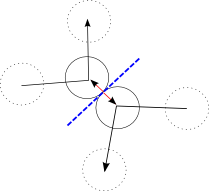
\includegraphics[height=2in]{figures/collision.png}
		\vskip5pt
		Need to keep them separated
		
	\pause
	\column{.5\textwidth}
	
	{\bf Standard method:}
	
	\begin{itemize}
	\item Time step to point of impact
	\pause
	\item Determine contact manifold
	\pause
	\item Apply penalty force/impulse to separate objects
	\pause
	\item Iterate until all collisions are resolved
	\end{itemize}
	\pause
	\vskip5pt
	+ Just like high school physics
	
\end{columns}
\end{frame}


\begin{frame}
\frametitle{Problems with typical collision methods}
Handling collisions this way is hard
\vskip5pt
\pause
\begin{itemize}
\item{-} Finding exact point/time of impact is expensive
\item{-} Contact manifolds can be difficult to classify
\item{-} Normal forces are ambiguous for curvy shapes
\item{-} Impulses are discontinuous; results in stiff system
\item{-} Penalty methods don't gaurantee separation
\item{-} Convergence properties not well understood
\item{-} Unclear how to handle sharp corners
\item{-} Discontinuity in simulation
\item{-} Complicated, ad-hoc
\end{itemize}
\pause
But can be made to work with enough hacking...
\end{frame}

\begin{frame}
\frametitle{There has got to be an easier way...}
\pause
Minimal requirement for physical plausibility
\vskip7pt
\begin{center}
\emph{At all times no two solids intersect}
\end{center}
\pause
\vskip15pt
Is this really all there is to it?

\end{frame}

\section{Constraint Based Collisions}
\begin{frame}
\frametitle{Constraint Based Impacts}
For any body $B_i$ with mass field $\varphi_i$, define the set:
\[ A_i = \kappa \iota \text{ supp } \varphi \]
\pause
So two solids, $A_i, A_j$, \emph{collide} at a configuration $q_i, q_j$ iff:
\[ \text{collide}(q_i A_i, q_j A_j) \Leftrightarrow \iota (q_i A_i \cap q_j A_j) \neq \emptyset \]
\pause
But,
\[ \iota ( q_i A_i \cap q_j A_j ) \neq \emptyset \Leftrightarrow \text{vol } q_i A_i \cap q_j A_j > 0 \]
\pause
Define
\[ C_{i,j}(q_i, q_j) \stackrel{def}{\equiv} \text{vol } q_i A_i \cap q_j A_j \]
And so we replace the impact forces with a system of differentiable holonomic inequality constraints:
\[ C_{i,j} \leq 0 \]
\end{frame}

\begin{frame}
\frametitle{Equations of motion revisited}
New problem:
\[ \text{minimize } \int \limits_{t_0}^{t_1} L(q, \dot{q}, t) dt \]
\[ \text{subject to } C_{i,j}(q_i, q_j) \leq 0 \:\:\: \forall t \in [t_0, t_1), i \neq j \]
\pause
Apply KKT conditions + Euler-Lagrange to get complementarity problem:
\[ \frac{d}{dt} \left( \frac{\partial T(\dot{q}_i)}{\partial \dot{q}_i} \right)
- \frac{\partial U(q, t)}{\partial q_i} + \alert<3>{\sum \limits_{j \neq i} \mu_{i,j} \frac{ \partial C_{i,j}(q_i, q_j)}{ \partial{q_i} }} = 0 \]
\[ \alert<3>{0 \leq \mu_{i,j} \perp -C_{i,j} \geq 0} \]
\pause
Exactly elastic collision response!
\vskip5pt
Slack variables are impulse forces
\end{frame}

\begin{frame}
\frametitle{Calculating $C_{i,j}$}
Need to compute:
\[ C_{i,j}(q_i, q_j) = \text{vol } q_i A_i \cap q_j A_j \]
\pause
Construct the \emph{indicator} on $A$
\[ \ind{A}(x) = \left \{ \begin{array}{cc}
1 & \text{if } x \in A \\
0 & \text{otherwise}
\end{array} \right. \]
\pause
Observe:
\begin{columns}
	\column{.5\textwidth}
		{\centering
		\[ \ind{A_i \cap A_j}(x) = \ind{A_i}(x) \ind{A_j}(x)  \]
		}
	
	\column{.5\textwidth}
		{\centering
		\[ \text{vol } A_i = \int \limits_{\R^d} \ind{A_i}(x) dx \]
		}
\end{columns}
\pause
So:
\[ C_{i,j}(q_i, q_j) = \int \limits_{\R^d} \ind{A_i}(q_i^{-1} x) \ind{A_j}(q_j^{-1} x) dx \]
\end{frame}

\begin{frame}
\frametitle{Calculating $C_{i,j}$ (cont.)}
\[ C_{i,j}(q_i, q_j) = \int \limits_{\R^d} \ind{A_i}(q_i^{-1} x) \ind{A_j}(q_j^{-1} x) dx \]
\pause
Push terms to one side:
\[ \int \limits_{\R^d} \ind{A_i}(x) \ind{A_j}(q_j^{-1} q_i x) dx \]
\pause
Substitute $q_j^{-1} q_i x \mapsto Rx - y$ and let $\widetilde{\ind{A_j}}(x) = \ind{A_j}(-x)$:
\[ \int \limits_{\R^d} \ind{A_i}(x) \widetilde{\ind{A_j}}(y - Rx) dx = 
\int \limits_{\R^d} \ind{A_i}(R^{-1} x) \widetilde{\ind{A_j}}(y - x) dx\]
\pause
So,
\[ C_{i,j}(q_i, q_j) = ((\ind{A_i} \circ R^{-1}) \star \widetilde{\ind{A_j}})(y) \]
\end{frame}

\section{Fourier Methods}
\begin{frame}
\frametitle{Fourier Methods}
Convolution? \invisible<1>{Take a Fourier transform!}
\[ C_{i,j}(q_i, q_j) = ((\ind{A_i} \circ R^{-1}) \star \widetilde{\ind{A_j}})(y)
\pause
= \mathcal{F}^{-1} \left ( (\widehat{\ind{A_i}} \circ R^{-1}) \overline{\widehat{\ind{A_j}}} \right )(y) \]
\pause
What about gradients? (ie $\frac{\partial C_{i,j}(q_i, q_j)}{\partial q_i}$)
\pause
\vskip5pt
\vskip5pt
\begin{columns}
	\column{.5\textwidth}
		{\centering
		Fix parameters $q_i = (R_i, t_i)$, 
		\[q_i x = R_i x + t_i \]
		\[q_i^{-1} = (R_i^{-1}, -R_i^{-1} t_i) \]
		\[q_j q_i^{-1} x = Rx - y\]
		}
	\column{.5\textwidth}
		\pause
		{\centering
		Solve for $R, y$,
		\[ R = R_j R_i^{-1} \]
		\[ y = t_j - R_j R_i^{-1} t_i \]
		}
\end{columns}
\pause
Need to compute $\frac{\partial C_{i,j}(R, y)}{\partial y}$, $\frac{\partial C_{i,j}(R, y)}{\partial R}$ then use chain rule
\vskip5pt
Or by symmetry: $C_{i,j}(q_i, q_j) = C_{j,i}(q_j, q_i)$
\end{frame}

\begin{frame}
\frametitle{Translational Gradient}
Start with the translational case first.
\vskip5pt
Let $y^k$ denote the $k^{th}$ component of $y$,\pause then
\begin{eqnarray*}
\frac{ \partial C_{i,j} }{ \partial y^k }
& = & \frac{ \partial }{ \partial y^k } \left( \:\: \int \limits_{\R^d} \widehat{\ind{A_i}}(R^{-1} \omega) \overline{\widehat{\ind{A_j}}(\omega)} e^{2 \pi i \inner{\omega}{y}} d \omega  \right ) \\
\pause 
...
& = & \int \limits_{\R^d} 
\alert<4>{2 \pi i \inner{\omega}{v^k}}
\widehat{\ind{A_i}}(R^{-1} \omega) \overline{\widehat{\ind{A_j}}(\omega)} e^{2 \pi i \inner{\omega}{y} } d \omega
\end{eqnarray*}
Where $v^k$ denotes the $k^{th}$ basis vector
\pause
\vskip5pt
Conclusion: Translational gradient is just a multiplier
\end{frame}

\begin{frame}
\frametitle{Rotational Gradient}
\newcommand{\rr}{\mathfrak{r}}
Parameterize $R = \exp( \mathfrak{r} )$, where $\rr \in \mathfrak{so}(d)$ with basis $\rr_{k,l}$ \vskip2pt
\hskip5pt{\small In otherwords $d \times d$ skew symmetric matrices, $\rr^T = -\rr$}
\pause
\begin{eqnarray*}
\frac{\partial C_{i,j}}{\partial \rr_{k,l}}  
& = &
 \frac{ \partial }{ \partial \rr_{k,l} } \left( \:\: 
	\int \limits_{\R^d} 
		\widehat{\ind{A_i}}(\exp(-\rr) \omega) 
		\overline{\widehat{\ind{A_j}}(\omega)} 
		e^{2 \pi i \inner{\omega}{y}} 
	d \omega
\right )\\
\pause
...
& = &
	\int \limits_{\R^d} 
		-\inner{ \alert<4>{\nabla \widehat{\ind{A_i}}(R^{-1} \omega)} }{ R^{-1} \rr_{k,l} \omega } \overline{\widehat{\ind{A_j}}(\omega)} e^{2 \pi i \inner{\omega}{y}} d \omega
\end{eqnarray*}
\pause
Not a Fourier multiplier.
\vskip5pt
\pause
But can be precalculated with $O(d)$ overhead:
\vskip5pt
\[ \frac{\partial}{\partial \omega^k} \widehat{\ind{A_i}}(\omega) = \mathcal{F}\left( -2 \pi i \inner{x}{v^k} \ind{A_i}\right)(\omega) \]
\end{frame}

\begin{frame}
\frametitle{Performance}
Fourier transform is neat, but what does it get us?
\vskip10pt
\pause
Full inverse Fourier transform complexity = brute force volume
\vskip2pt
\hskip10pt {\small Though the derivative formulas are cute...}
\vskip2pt
\hskip10pt {\small And we do get slightly better cache coherency...}
\vskip10pt
\pause
But do we really need the whole spectrum?
\pause
\vskip15pt
\begin{center}
\alert{\bf {\Huge NO!}}
\end{center}
\pause
\vskip15pt
Since Fourier series exhibit exponential convergence for suitably regular functions, only need about $O(-log(h))$ terms to get $O(h)$ accuracy (in the $L^1$ norm).
\vskip10pt
\pause
Dramatically reduces space and time complexity
\end{frame}

\begin{frame}
\frametitle{Convergence}
Rate of convergence, number of Fourier terms vs. $L^1$ error, (log-log plot)
\begin{center}
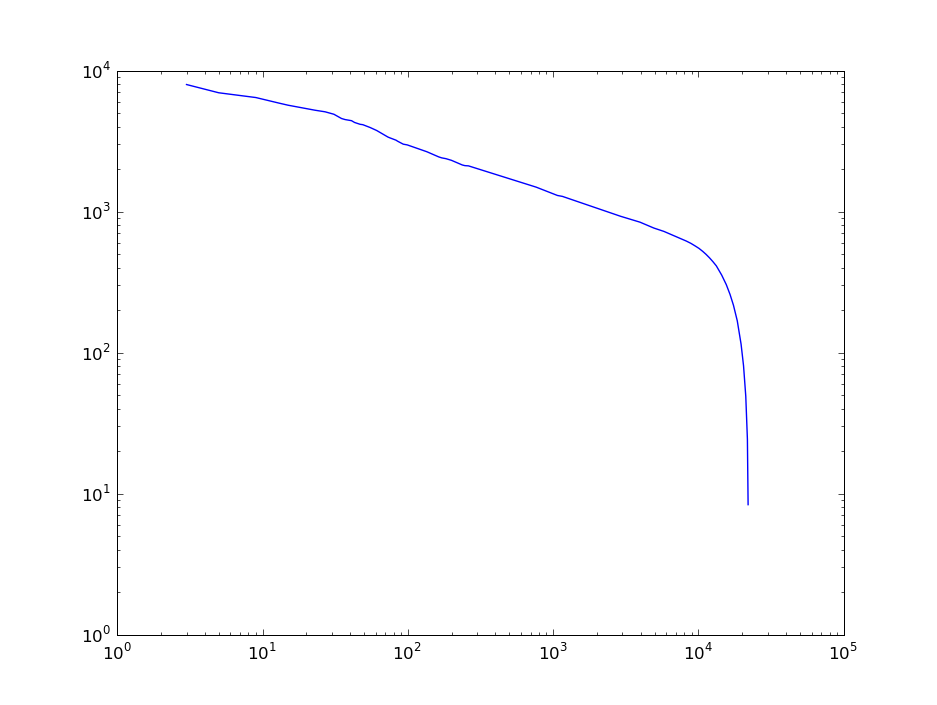
\includegraphics[height=2.5in]{figures/trunc_errors.png}
\end{center}
\end{frame}

\begin{frame}
\frametitle{Convergence}
Qualitative effects of cutoff (full spectrum has 22185 terms)
\begin{center}
\begin{tabular}{ccc}

\includegraphics[height=1in]{figures/trunc_exact.png} &

\includegraphics[height=1in]{figures/trunc_16.png} &
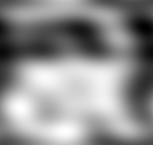
\includegraphics[height=1in]{figures/trunc_32.png} \\
Exact &
16 &
32 \\
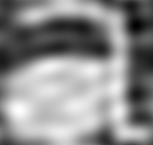
\includegraphics[height=1in]{figures/trunc_64.png} &
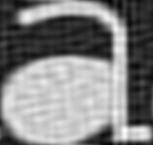
\includegraphics[height=1in]{figures/trunc_256.png} &
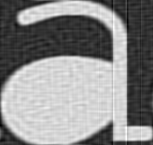
\includegraphics[height=1in]{figures/trunc_1024.png} \\
64 &
256 &
1024 \\
\end{tabular}
\end{center}
\end{frame}

\section{Numerical Issues}
\begin{frame}
\frametitle{Truncated Spectra}
Henceforth $d = 2$
\vskip5pt
Want: An efficient way to represent truncated spectrum
\vskip2pt
\hskip10pt Need to deal with rotations too
\vskip5pt
Obvious answer: Polar coordinates
\vskip5pt
Pick $\omega_r = \sqrt{\omega_x^2 + \omega_y^2}$, $\omega_\theta = \tan^{-1} \frac{y}{x}$
\[ \widehat{f}(\omega_x, \omega_y) \mapsto \widehat{f}^p(\omega_r, \omega_\theta) \]
\pause
Rotation $\mapsto$ Cyclic shift in $\theta$

Differentiation formulas still work, just do change of variables

Seems easy, right?
\pause
\begin{center}

\includegraphics[width=.5in]{figures/trollface.png} \emph{Problem?}
\end{center}
\end{frame}

\begin{frame}
\frametitle{Discrete Cartesian to Polar Conversion}
Can't do this exactly!
\begin{center}
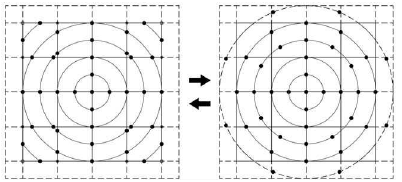
\includegraphics[height=1.7in]{figures/polar_chirik.png}

{\tiny Figure from Chirikjian 2003}
\pause
\end{center}
\begin{columns}
	\column{.9\textwidth}
		Reason: \emph{Only nontrivial discrete subgroups of $SE(2)$ are 17 plane tiling groups!} 
	\column{.1\textwidth}	
		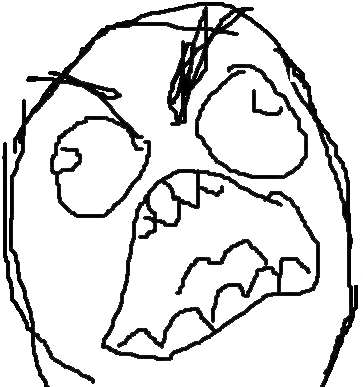
\includegraphics[height=.5in]{figures/fffuuuu.png}
\end{columns}
\pause
{\small So unless you are happy with a hexagonal grid with 6 rotational samples, forget about doing this losslessly! }
\end{frame}

\begin{frame}
\frametitle{Bresenham Interpolation}
Approximation is a fact of life -- deal with it
\vskip2pt
\hskip10pt {\small Might as well do it fast}
\vskip2pt
\pause
Idea: Do circle drawing in reverse, use Bresenham's algorithm
\begin{columns}

	\column{.4\textwidth}
		\begin{center}
		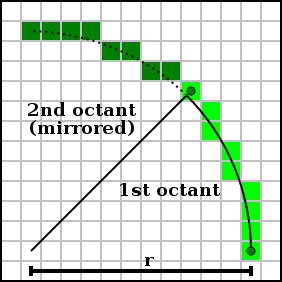
\includegraphics[height=1.4in]{figures/wiki_bresenham.png}

		{\tiny Figure from Wikipedia, 2010}
		\end{center}
		
	\column{.6\textwidth}
		\pause
		\begin{itemize}
			\item Sample $r$ at uniform increments
			\item For each $r$, trace a circle centered at the origin
			\item Store $8r + 4$ radial samples in array
			\item Interpolate to uniform radial samples
			\item Append to store
		\end{itemize}
\end{columns}
\pause
Minimal storage, uses only integer arithmetic 
\includegraphics[height=.5in]{figures/everything_went_better_than_expected.jpg}
\end{frame}

\begin{frame}
\frametitle{Gibbs Phenomenon}
Truncating Fourier series causes ringing artifacts at boundaries
\vskip2pt
\hskip10pt {\small Intuitively, same as low pass filtering high curvature}
\begin{center}
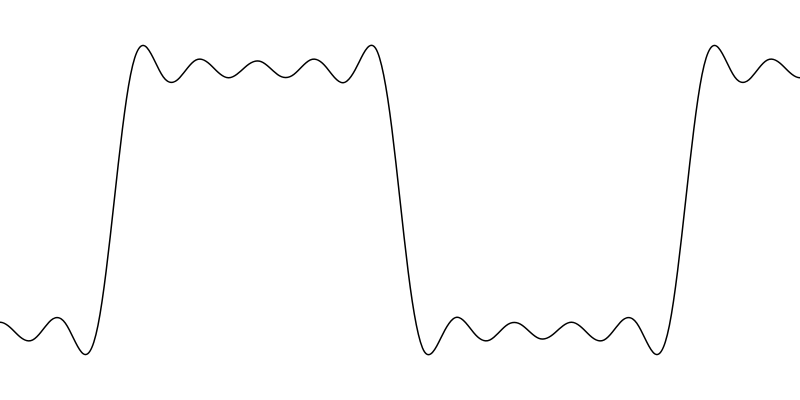
\includegraphics[height=1.2in]{figures/wiki_gibbs.png}

{\tiny Figure from Wikipedia, 2010}
\end{center}
\pause
But we don't care, just need separation between interior and exterior.
\vskip5pt
So pick some cutoff threshold; values above are in, below are out
\end{frame}

\begin{frame}
\frametitle{Optimal Thresholding}
Given a region $R \subset \R^d$ and set $A \subseteq R$ approximated by $f$, define quality, $Q_T$, of threshold $T$
\[ Q_T = \text{vol } \{ x \in R | f(x) > T \Leftrightarrow x \in A \} \]
\emph{Intuitively, number of points where threshold gives the right answer}

Want to find optimal $T$
\[ T = \mathop{\text{argmax}}_{T' \in \R} Q_{T'} \]
Seems hard to estimate $T$ analytically
\pause
\vskip5pt
But in practice can compute $T$ combinatorially given $f, A, R$
\end{frame}

\begin{frame}[fragile]
\frametitle{Optimal Thresholding Algorithm}
\begin{lstlisting}
v = []
for x in R:
    v.append( (f(x), A(x)) )
v.sort()

fv, Av = unzip(v)
Q = foldl(Av, +, 0) + foldr(Av, +, 0)

return max(zip(Q, fv)).second
\end{lstlisting}

\vskip10pt
Greedy/DP method

\vskip10pt
Takes $O(n \log(n))$ time, uses $O(n)$ space
\end{frame}

\begin{frame}
\frametitle{Low Pass Filter/Thresholding Results}
\begin{center}
\centering
\begin{tabular}{|c|c|c|}
\hline
Exact Indicator & 
Fourier Truncation & 
Optimal Cutoff \\
\hline

\includegraphics[height=.5in]{figures/fig_ind0.png} & 

\includegraphics[height=.5in]{figures/fig_ift0.png} & 

\includegraphics[height=.5in]{figures/fig_cut0.png} \\
\hline

\includegraphics[height=.5in]{figures/fig_ind1.png} & 

\includegraphics[height=.5in]{figures/fig_ift1.png} & 
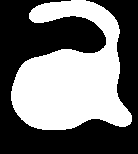
\includegraphics[height=.5in]{figures/fig_cut1.png} \\
\hline

\includegraphics[height=.5in]{figures/fig_ind2.png} & 

\includegraphics[height=.5in]{figures/fig_ift2.png} & 

\includegraphics[height=.5in]{figures/fig_cut2.png} \\
\hline

\includegraphics[height=.5in]{figures/fig_ind3.png} & 

\includegraphics[height=.5in]{figures/fig_ift3.png} & 

\includegraphics[height=.5in]{figures/fig_cut3.png} \\
\hline
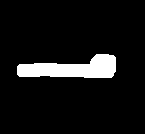
\includegraphics[height=.5in]{figures/fig_ind4.png} & 

\includegraphics[height=.5in]{figures/fig_ift4.png} & 
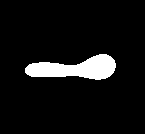
\includegraphics[height=.5in]{figures/fig_cut4.png} \\
\hline
\end{tabular}

Radius 14 cutoff, 777 terms
\end{center}
\end{frame}

\begin{frame}
\frametitle{Putting it together}
Let $\hat{f_A}$ be the approximate Fourier series for $\ind{A}$
\vskip5pt
Then:
\begin{eqnarray*}
C_{i,j}(\rho, \theta, \phi) & = & -T +
	\sum \limits_{r=2}^{N_R}
		 \sum \limits_{t = 1}^{8 r + 4} 
			\widehat{f_{A_i}} \left( r, \phi \frac{d t}{d \theta} + t \right) 
			\overline{\widehat{f_{A_j}}} \left( r, t \right) \\
& ... &	 	\exp \left( 
				\frac{2 \pi i}{N} \rho r 
				\cos \left( 
						t \frac{d \theta}{dt} + \theta 
				\right) 
			\right)
			r \frac{d t}{d \theta}
\end{eqnarray*}
Where:
\begin{columns}
	\column{.5\textwidth}
		\[ q_j q_i^{-1} = (R, y) \]
		\[ y = \rho( \cos(\theta) v^x + \sin(\theta) v^y) \]
		\[ R = \exp(\phi \mathfrak{r}_{0,1}) \]
		
	\column{.5\textwidth}
		\[ dt = 8r + 4 \]
		\[ d\theta = 2 \pi \]
\end{columns}
\pause
\vskip5pt
\emph{Protip: Can early out using the rearrangement inequality}
\end{frame}

\begin{frame}
\frametitle{Prototype Physics Code}

Basic implementation so far, just uses implicit Euler.

\hskip10pt Doesn't solve for $\mu$ correctly (currently set to constant)

\vskip15pt
\begin{columns}

	\column{.5\textwidth}
		\begin{center}
		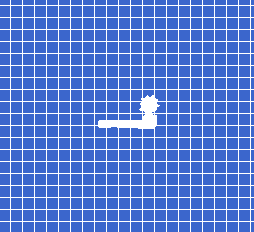
\includegraphics[width=1.8in]{figures/screenshot.png}
		\end{center}
		
	\column{.5\textwidth}
		Features:
		\begin{itemize}
			\item OpenGL GUI
			\item Written 100\% in Python
			\item Reasonable performance (though certainly not fast)
			\item Arbitrary shapes/mass fields supported
		\end{itemize}
\end{columns}

\vskip15pt
Download Link:
\begin{center}
http://github.com/mikolalysenko/Collisions
\end{center}
\end{frame}

\begin{frame}
\frametitle{To Do}
\begin{itemize}
\item Analysis is still very incomplete
\item Need to implement a proper solver for physics system
\item Benchmarks, etc.
\item More development/write ups needed
\end{itemize}
\end{frame}

\begin{frame}
\frametitle{References}
Stewart. "Rigid-body dynamics with friction and impact." SIAM Review, vol. 42 (issue 1), pp. 3-39, 2000.
\vskip10pt
Chirikijian and Kyatkin. "Engineering Applications of Noncommutative Harmonic Analysis." CRC Press.  2001
\vskip10pt
Baraff. "An Introduction to Physically Based Modelling." ACM SIGGRAPH. 1997
\vskip10pt
Arnold. "Mathematical Methods of Classical Mechanics." Springer. 1976.
\end{frame}

\end{document}

